%!TEX root = main.tex
%
% ToposOfGraphs.tex
%

\section{Worked Example: The Topos of Graphs}

In this section we explore the topos of graphs. Let $\mathbf{C}$ be the category given by
\[ \begin{tikzcd}
 V \arrow[r, bend left, "s"] \arrow[r, bend right, "t"] & E
\end{tikzcd} \]
and let $\mathscr{E} = \mathbf{Sets}^{\mathbf{C}^{op}}$. The objects of $\mathscr{E}$ may be viewed as graphs. Note that $\mathscr{E}$ is a connected topos because the terminal presheaf $1$ cannot be written as a non-trivial coproduct $1 = X + Y$. The topos $\mathscr{E}$ furthermore has a structure morphism to $\mathbf{Sets}$, namely
\[ \gamma : \mathscr{E} \to \mathbf{Sets}, \qquad \gamma_*(X) = \Hom_{\mathscr{E}}(1,X), \; \gamma^*(S) = \Delta S. \]
A connected object in $\mathscr{E}$ is a connected graph. Every $X \in \mathscr{E}$ thus has a decomposition $X = \sum_{i \in I} X_i$ into its connected components. So we have a functor
\[ \pi_0 : \mathscr{E} \to \mathbf{Sets}, \qquad \sum_{i \in I} X_i \mapsto I. \]
This functor $\pi_0$ is left adjoint to the constant presheaf functor $\Delta$, so
\[ \pi_0 \dashv \gamma^* \dashv \gamma_*. \]
Note that the subobject classifier $\Omega$, like for all presheaf categories, is given by
\begin{align*}
\Omega(V) &= \{ \text{sieves on } V \} = \{\emptyset, \mathbf{y}V \}, \\
\Omega(E) &= \{ \text{sieves on } E \} = \{\emptyset, \{s\}, \{t\}, \{s,t\}, \mathbf{y}E \}, \\
\Omega(s) &= \text{ pullback the sieve by } s, \\
\Omega(t) &= \text{ pullback the sieve by } t.
\end{align*}
So in a picture, the graph $\Omega$ looks like as in Figure 1.

\begin{figure}
\centering
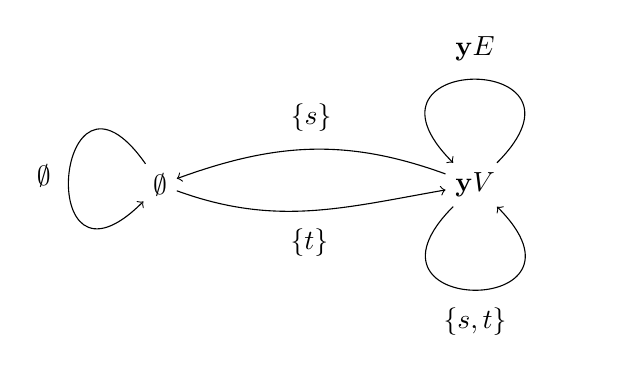
\begin{tikzpicture}
 \node (x) at (-2,0) {$\emptyset$};
 \node (y) at ( 2,0) {$\mathbf{y}V$};
 \path (x) edge [out=125, in=225, looseness=0.8, loop, distance=2cm, ->] node[left= 3pt] {$\emptyset$} (x);
 \path (y) edge [out= 45, in=135, looseness=0.8, loop, distance=2cm, ->] node[above=3pt] {$\mathbf{y}E$} (y);
 \path (y) edge [out=225, in=315, looseness=0.8, loop, distance=2cm, ->] node[below=3pt] {$\{s,t\}$} (y);
 \path (x) edge [out=340, in=190, ->] node[below=3pt] {$\{t\}$} (y);
 \path (y) edge [out=160, in=20, ->] node[above=3pt] {$\{s\}$} (x);
\end{tikzpicture}
\caption{The subobject classifier of $\mathscr{E}$}
\end{figure}

The subobject classifier is thus given by
\[ \text{true} : 1 \to \Omega, \qquad v \mapsto \mathbf{y}V, \; e \mapsto \mathbf{y}E. \]
If $X \in \mathscr{E}$ and $S \subseteq X$ a subgraph, then the classifying map $\chi_S : X \to \Omega$ works as follows:
\begin{itemize}
	\item For each vertex $v \in X(V)$:
	\begin{itemize}
		\item If $v \not\in S(V)$, then $\chi_S(V)(v) = \emptyset$.
		\item If $v \in S(V)$, then $\chi_S(V)(v) = \mathbf{y}V$.
	\end{itemize}
	\item For each edge $e \in X(E)$:
	\begin{itemize}
		\item If $e \in S(E)$, then $\chi_S(E)(e) = \mathbf{y}E$.
		\item Else (we know that $e \not\in S(E)$):
		\begin{itemize}
			\item If $X(s)(e), X(t)(e) \in S(V)$, then $\chi_S(E)(e) = \{s,t\}$ (the edge is not in $S$, but both its source and target vertices are).
			\item Else if $X(s)(e) \in S(V)$, $X(t)(e) \not\in S(V)$, then $\chi_S(E)(e) = \{s\}$ (the edge is not in $S$, and only its source vertex is in $S$).
			\item Else if $X(s)(e) \not\in S(V)$ $X(t)(e) \in S(V)$, then $\chi_S(E)(e) = \{t\}$ (the edge is not in $S$, and only its target vertex is in $S$).
			\item Else $\chi_S(E)(e) = \emptyset$.
		\end{itemize}
	\end{itemize}
\end{itemize}
Basically, this works as you'd expect for subgraphs in a picture. You can leave out edges in a subgraph, but keep some of its target and source vertices.
The negation operator $\neg : \Omega \to \Omega$ is a natural transformation with two components $\neg_V : \Omega V \to \Omega V$ and $\neg_E : \Omega E \to \Omega E$. They are defined as (cf. page 56 of Maclane\&Moerdijk)
\[ \neg_V : \Omega V \to \Omega V, \qquad \neg_V(\emptyset) = \mathbf{y}V, \; \neg_V(\mathbf{y}V) = \emptyset, \]
and
\[ \neg_E : \Omega E \to \Omega E, \]
explicitly calculated as
\begin{align*}
\neg_E(\emptyset) &= \mathbf{y}E, \\
\neg_E(\mathbf{y}E) &= \emptyset, \\
\neg_E(\{s\}) &= \emptyset\\
\neg_E(\{t\}) &= \emptyset\\
\neg_E(\{s,t\}) &= \emptyset\\
\end{align*}
Now let $\mathscr{E}_{lcf}$ be the Boolean topos of locally constant objects of $\mathscr{E}$. Since $\mathscr{E}_{lcf}$ is Boolean, its subobject classifier is given by
\[ \Omega_{lcf} = 1 + 1 \]
generated by the morphisms
\[ \text{true} : 1 \to \Omega, \qquad \text{false} = \neg \circ \text{true} : 1 \to \Omega. \]
So $\Omega_{lcf}$ looks like Figure 2.

\begin{figure}
\centering
\begin{tikzpicture}
 \node (x) at (-2,0) {$\emptyset$};
 \node (y) at ( 2,0) {$\mathbf{y}V$};
 \path (x) edge [out=125, in=225, looseness=0.8, loop, distance=2cm, ->] node[left= 3pt] {$\emptyset$} (x);
 \path (y) edge [out= 45, in=135, looseness=0.8, loop, distance=2cm, ->] node[above=3pt] {$\mathbf{y}E$} (y);
\end{tikzpicture}
\caption{The subobject classifier of $\mathscr{E}_{lcf}$}
\end{figure}

Recall that $C_n \in \mathscr{E}_{lcf}$ is the cyclic graph with $n$ vertices and $n$ edges.

\begin{claim}
Let $\mathbf{G}$ be the full subcategory of $\mathbf{I}$ whose objects are Galois. Then every object of $\mathbf{G}$ is of the form $(C_n,e)$ for some $n > 0$.
\end{claim}
\begin{proof}
Write $C_n(V) = \{v_0,\ldots,v_{n-1}\}$ and $C_n(E) = \{e_0,\ldots,e_{n-1}\}$. Then $\Aut(C_n) = \Z/n\Z$, with action given by $m \cdot e_j = e_{j + m \bmod{n}}$. Hence $\Aut(C_n) \cong p^*(C_n)$, so $\mathbf{G}$ certainly contains all the $(C_n,e)$. Conversely suppose that $(A,e) \in \mathbf{G}$. Let $\varphi : A \times U \to \Delta n \times U$ be an isomorphism over $U$, where $U \to 1$ has global support. Note that $\# A = \# \Delta n = n$. Let $v \in A$ be a vertex. Let $\partial^+(v)$ be the number of incoming edges into the vertex $v$. Assume that $\partial^+(v) = 0$. Then for all $(v,u) \in A \times U$ we also have $\partial^+(v,u) = 0$. However $\varphi(v,u) = (v_j,u)$ for some $v_j \in C_n$, and $\partial^+(v_j,u) > 0$ for some $u \in U(V)$. This is in contradiction with $\partial^+(v,u) = 0$ for all $u \in U(V)$. So we conclude that $\partial^+(v) > 0$ for all $v \in A(V)$. This forces $\partial^+(v) = 1$ for all $v \in A(V)$, because $n = \sum_{v \in A(V)} \partial^+(v)$. Since we didn't use the fact that these edges are incoming, the same argument shows that the number of outgoing edges is also $1$ for each $v \in A(V)$. Finally, since $A$ is connected we may conclude that $A = C_n$.
\end{proof}

So the cycles form a cofinal subcategory of $\mathbf{I}$. Thus we may conclude that
\[ \pi_1(\mathscr{E}, p) = \lim_{\leftarrow \mathbf{G}} \Aut(C_n) \cong \lim_{\leftarrow n} \Z/n\Z = \widehat{\Z}. \]
